\documentclass{ximera}


\graphicspath{
  {./}
  {ximeraTutorial/}
  {basicPhilosophy/}
}

\newcommand{\mooculus}{\textsf{\textbf{MOOC}\textnormal{\textsf{ULUS}}}}


\usepackage{tkz-euclide}\usepackage{tikz}
\usepackage{tikz-cd}
\usetikzlibrary{arrows}
\tikzset{>=stealth,commutative diagrams/.cd,
  arrow style=tikz,diagrams={>=stealth}} %% cool arrow head
\tikzset{shorten <>/.style={ shorten >=#1, shorten <=#1 } } %% allows shorter vectors

\usetikzlibrary{backgrounds} %% for boxes around graphs
\usetikzlibrary{shapes,positioning}  %% Clouds and stars
\usetikzlibrary{matrix} %% for matrix
\usepgfplotslibrary{polar} %% for polar plots
\usepgfplotslibrary{fillbetween} %% to shade area between curves in TikZ
\usetkzobj{all}
\usepackage[makeroom]{cancel} %% for strike outs
%\usepackage{mathtools} %% for pretty underbrace % Breaks Ximera
%\usepackage{multicol}
\usepackage{pgffor} %% required for integral for loops



%% http://tex.stackexchange.com/questions/66490/drawing-a-tikz-arc-specifying-the-center
%% Draws beach ball
\tikzset{pics/carc/.style args={#1:#2:#3}{code={\draw[pic actions] (#1:#3) arc(#1:#2:#3);}}}



\usepackage{array}
\setlength{\extrarowheight}{+.1cm}
\newdimen\digitwidth
\settowidth\digitwidth{9}
\def\divrule#1#2{
\noalign{\moveright#1\digitwidth
\vbox{\hrule width#2\digitwidth}}}
























%%This is to help with formatting on future title pages.
\newenvironment{sectionOutcomes}{}{}


\title{Law of Cosine}

\begin{document}

\begin{abstract}
extending Pythagorus
\end{abstract}
\maketitle







In the diagram below, we drop an \textbf{altitude} from the top corner (angle $C$). This altitude (length $h$) is perpendicular to the opposite side, forming two right triangles inside the acute triangle. \\




\begin{image}[3in]
    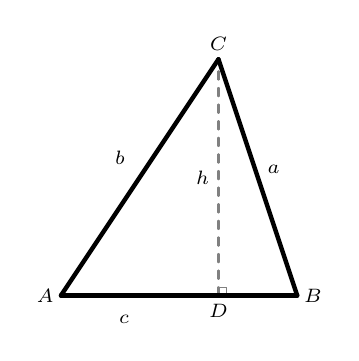
\begin{tikzpicture}[line cap=round]


    \draw [thick, dashed, gray] (2,0) -- (2,3);
    \draw [thin, gray] (2,0.1) -- (2.1,0.1);
    \draw [thin, gray] (2.1,0) -- (2.1,0.1);

	\draw [ultra thick] (0,0) -- (3,0);
	\draw [ultra thick] (3,0) -- (2,3);
	\draw [ultra thick] (0,0) -- (2,3);

 	


	\draw (2.7,1.6) node {\scriptsize{$a$}};
	\draw (0.75,1.75) node {\scriptsize{$b$}};
	\draw (0.8,-0.3) node {\scriptsize{$c$}};
	\draw (1.8,1.5) node {\scriptsize{$h$}};


	\draw (-0.2,0) node {\scriptsize{$A$}};
	\draw (3.2,0) node {\scriptsize{$B$}};
	\draw (2,3.2) node {\scriptsize{$C$}};
	\draw (2,-0.2) node {\scriptsize{$D$}};


    \end{tikzpicture}
  \end{image}




\begin{notation} \textbf{\textcolor{purple!85!blue}{Points, Line Segments, and Lengths}}  \\

If $A$ and $D$ are two points, then 

\begin{itemize}
\item the actual line segment itself connecting $A$ and $D$ is denoted as $\overline{AD}$. 
\item the length of this line segment is denoted as $m(\overline{AD})$.  $m$ stands for measurement.
\item If $A$ is a point, which is serving as the vertex of an angle, then the angle is denoted by $\measuredangle A$.
\end{itemize}
\end{notation}





From the right triangle on the left in the diagram, we can see that $\cos(\measuredangle A) = \frac{m(\overline{AD})}{b}$ or $m(\overline{AD}) = b \cos(\measuredangle A)$. \\


\textbf{Note:} When it is clear, the angle sign is almost always dropped. \\


From the right triangle on the left in the diagram, we can see that $\cos(A) = \frac{m(\overline{AD})}{b}$ or $m(\overline{AD}) = b \cos(A)$.


Subtracting this from $m(\overline{AB})$, gives us $m(\overline{DB}) = c - b \cos(A)$.


From the right triangle on the left in the diagram, we can see that $\sin(A) = \frac{h}{b}$ or $h = b \sin(A)$.




From the right triangle on the right in the diagram, the Pythagorean Theorem gives us $a^2 = (b \sin(A))^2 + (c - b \cos(A))^2$.


Multiplying everything out gives


\[    a^2 = b^2 \sin^2(A) +  c^2  - 2 b c \cos(A) + b^2 \cos^2(A)  \]


\[    a^2 = b^2 \sin^2(A) + b^2 \cos^2(A) +  c^2  - 2 b c \cos(A)   \]


\[    a^2 = b^2 (\sin^2(A) + \cos^2(A)) +  c^2  - 2 b c \cos(A)   \]


\[    a^2 = b^2  +  c^2  - 2 b c \cos(A)   \]












\begin{theorem}  \textbf{\textcolor{green!50!black}{Law of Cosines}}  \\



For any trinagle with angles $A$, $B$, and $C$, and opposite sides $a$, $b$, and $c$, respectively, 


\[    a^2 = b^2  +  c^2  - 2 b c \cos(A)   \]

\[    b^2 = a^2  +  c^2  - 2 a c \cos(B)   \]

\[    c^2 = a^2  +  b^2  - 2 a b \cos(C)   \]


\end{theorem}










\begin{example} Triangle \\

Suppose we have a triangle with $a=6$, $b=9$, and $c=11$. Approximate the measurement of angle $A$.

\[    6^2 = 9^2  +  11^2  - 2 \cdot 9 \cdot 11 \cos(A)   \]


\[    \frac{36 - 81 - 121}{- 2 \cdot 9 \cdot 11} =    \cos(A)   \]

\[  \answer[tolerance=0.001]{0.83838383} \approx \cos(A)  \]


\[ A \approx \cos^{-1}(0.83838383)  \approx \answer[tolerance=0.01]{33.030}^{\circ}   \]


\end{example}











\begin{center}
\textbf{\textcolor{green!50!black}{ooooo-=-=-=-ooOoo-=-=-=-ooooo}} \\

more examples can be found by following this link\\ \link[More Examples of Triangles]{https://ximera.osu.edu/csccmathematics/precalculus2/precalculus2/generalTriangles/examples/exampleList}

\end{center}








\end{document}
